\input{../preamble.tex}

\lecturenumber{14}
\title{Memory Allocation}
\version{1.0.0}

\begin{document}

\begin{frame}[plain, noframenumbering]
    \titlepage
\end{frame}

\begin{slide}

    \slidetitle{Static Allocation is the Simplest Strategy}

    Create a fixed size allocation in your program

    \leftspace{}e.g. \mintinline{c}{char buffer[4096];}
    \medskip

    When the program loads, the kernel sets aside that memory
    for you
    \medskip

    That memory exists as long as your process does, no need to free

\end{slide}

\begin{slide}

    \slidetitle{Dynamic Allocation is Often Required}

    You may only conditionally require memory

    \leftspace{}Static allocations are sometimes wasteful
    \medskip

    You may not know the size of the allocation

    \leftspace{}Static allocations need to account for the maximum size
    \medskip

    Where do you allocate memory?

    \leftspace{}You can either allocate on the stack or on the heap

\end{slide}

\begin{slide}

	\slidetitle{What we have covered so far}
	
	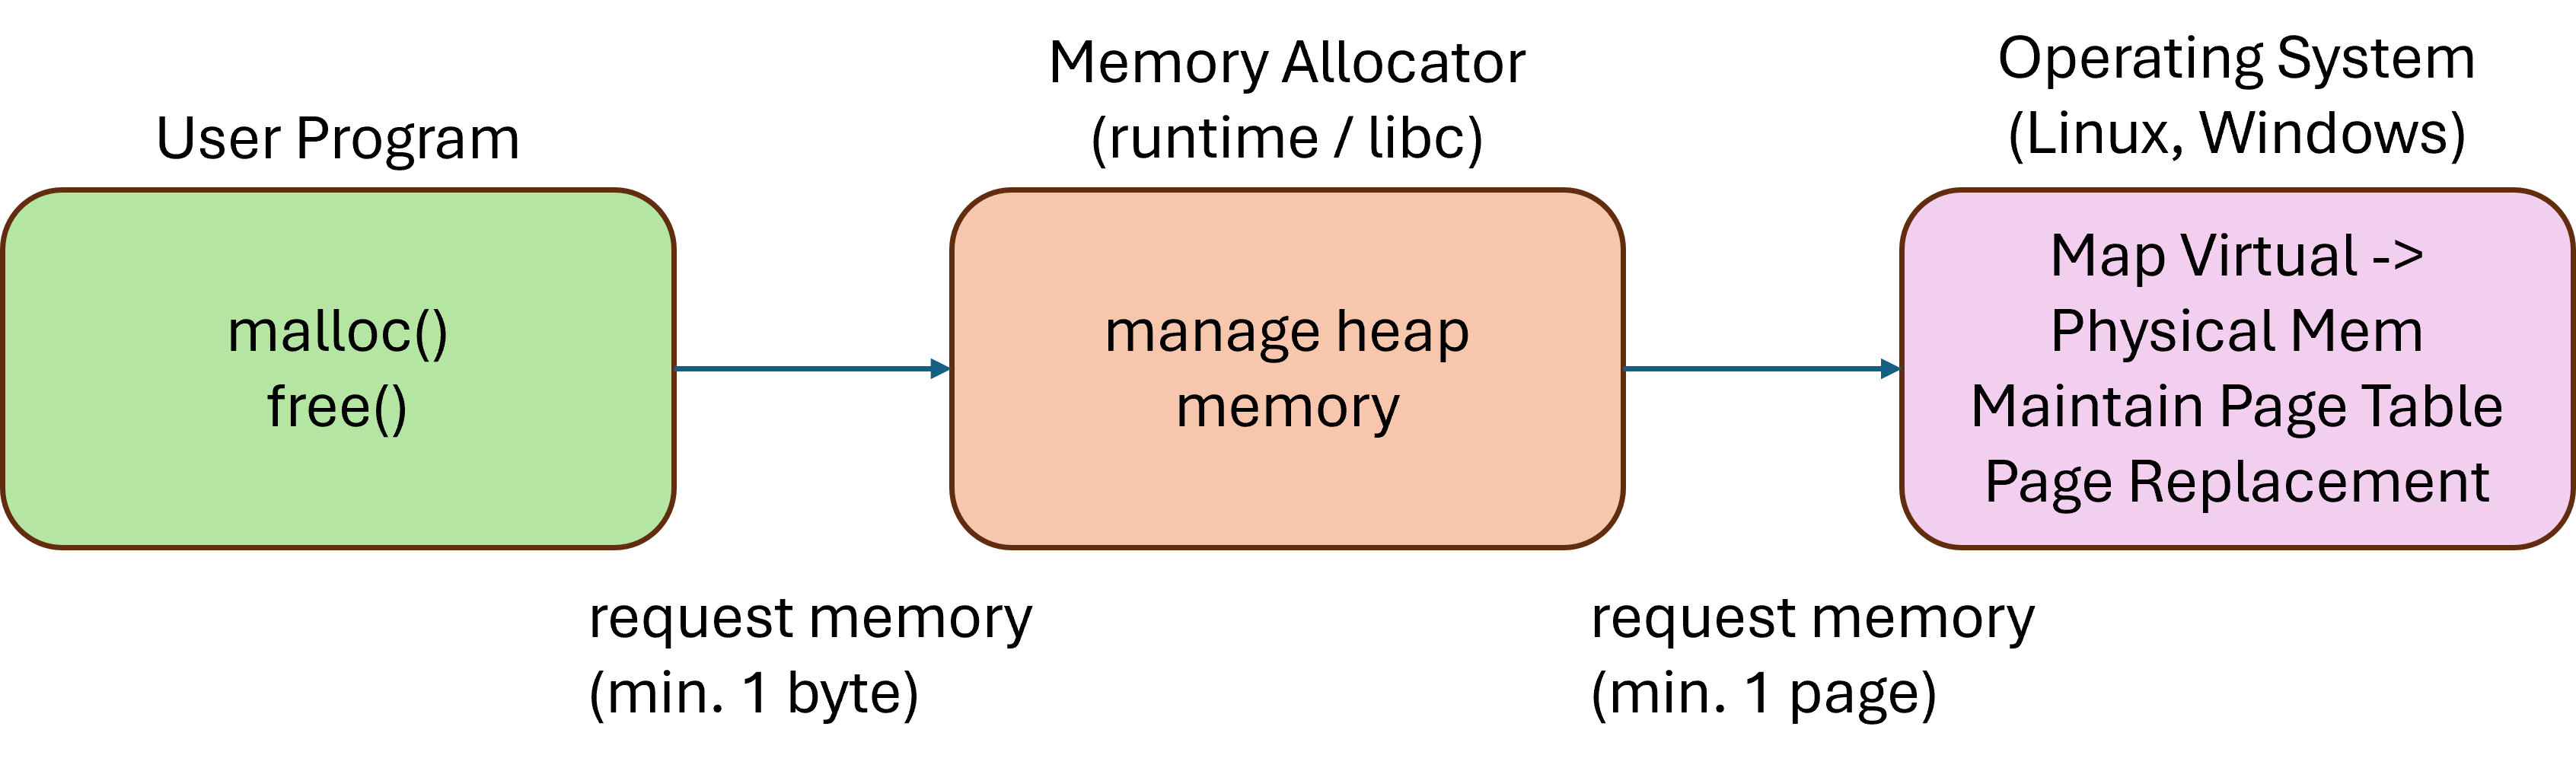
\includegraphics[width=120mm]{class-summary.png}
	
\end{slide}

\begin{slide}

    \slidetitle{Variable sized allocation}
	
	Given a block of memory, how do we allocate it to satisfy various memory allocation requests?
	
	\bigskip
	
	This problem must be solved in the C library
	\begin{itemize}
		\item Allocates one or more pages from kernel via \texttt{brk/sbrk} or \texttt{mmap} system calls
		\item Gives out smaller chunks to user programs via malloc
	\end{itemize}
	
	\bigskip
	
	This problem also occurs in the kernel
	\begin{itemize}
		\item Kernel must allocate memory for its internal data structures
	\end{itemize}

\end{slide}

\begin{slide}

	\slidetitle{Variable sized allocation: headers}
	
	Consider a simple implementation of malloc
	\bigskip
	
	Every allocated chunk has a header with info like size of chunk
	\bigskip
	
	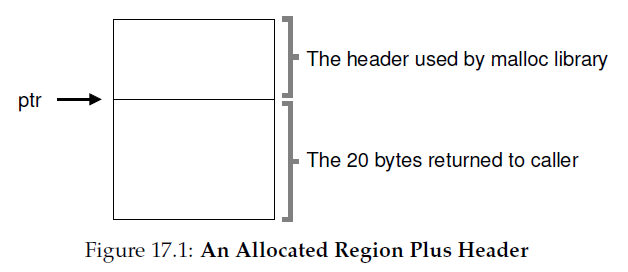
\includegraphics[width=50mm]{malloc-header.png}

\end{slide}

\begin{slide}

	\slidetitle{Free List}
	
	\vspace{-10mm}
	
	\begin{minipage}[t]{0.45\textwidth}
        \vspace{0pt}\par
		
		\vspace{8mm}
		
		Free space is managed as a list
		\medskip
		
		\begin{itemize}
			\item Pointer to the next free chunk is embedded within the free chunk
		\end{itemize}
		
		\bigskip
		
		The library tracks the head of the list
		\medskip
		\begin{itemize}
			\item Allocations happen from the head
		\end{itemize}
		
	\end{minipage}
	\hfill
	\begin{minipage}[t]{0.45\textwidth}
        \vspace{0pt}\par
		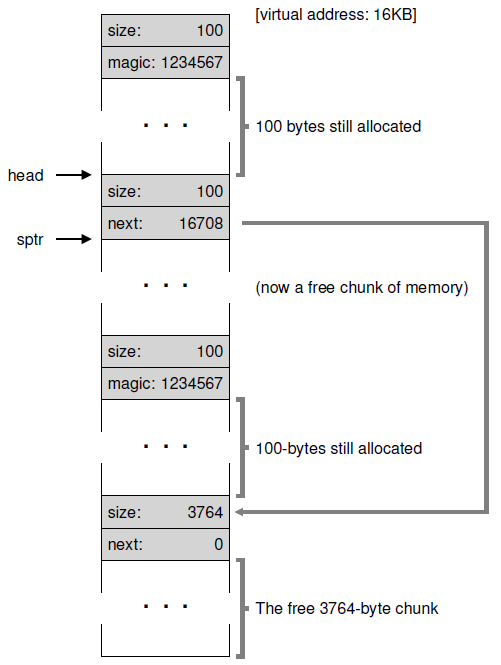
\includegraphics[width=50mm]{malloc-free-list.png}
	\end{minipage}

\end{slide}

\begin{slide}

	\slidetitle{Splitting and Coalescing}
	
	\vspace{-10mm}
	
	\begin{minipage}[t]{0.45\textwidth}
        \vspace{0pt}\par
		
		\vspace{8mm}
		
		Suppose all the three chunks are freed
		\bigskip
		
		The list now has a bunch of free chunks that are adjacent
		\bigskip
		
		A smart algorithm would merge them all into a bigger free chunk
		\bigskip
		
		Must split and coalesce free chunks to satisfy variable sized requests
		
	\end{minipage}
	\hfill
	\begin{minipage}[t]{0.45\textwidth}
        \vspace{0pt}\par
		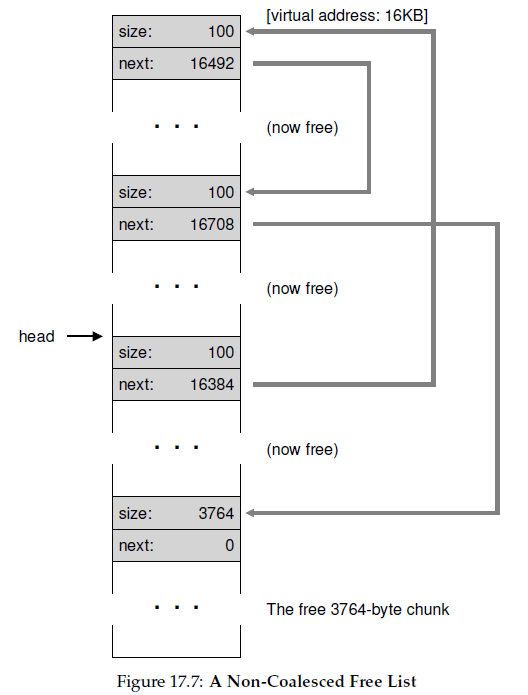
\includegraphics[width=50mm]{buddy-allocator-combined.png}
	\end{minipage}
	\end{slide}

\begin{slide}

    \slidetitle{Fragmentation is a Unique Issue for Dynamic Allocation}

    You allocate memory in different sized contiguous blocks

    \leftspace{}Compaction is not possible and every allocation decision is
    permanent
    \medskip

    A fragment is a small contiguous block of memory that cannot handle an
    allocation

    \leftspace{}You can think of it as a ``hole'' in memory, wasting space
    \medskip

    There are 3 requirements for fragmentation
    \begin{enumerate}
        \item Different allocation lifetimes
        \item Different allocation sizes
        \item Inability to relocate previous allocations  
    \end{enumerate}

\end{slide}

\begin{slide}
    
    \slidetitle{There's Internal and External Fragmentation}

    External fragmentation occurs when you allocate different sized blocks

    \leftspace{}There's no room for an allocation between the blocks

    \begin{center}
    \begin{tikzpicture}[node distance=0mm and 0mm]
      \node[draw,rectangle,minimum width=50,minimum height=30,fill=red]
        (a0) {};
      \node[draw,rectangle,minimum width=30,minimum height=30]
        (a1) [right=of a0] {};
      \node[draw,rectangle,minimum width=20,minimum height=30,fill=red]
        (a2) [right=of a1] {};
      \node[draw,rectangle,minimum width=60,minimum height=30]
        (a3) [right=of a2] {};
    \end{tikzpicture}
    \end{center}

    Internal fragmentation occurs when you allocate fixed sized blocks

    \leftspace{}There's wasted space within a block

    \begin{center}
    \begin{tikzpicture}[node distance=0mm and 0mm]
      \node[draw,rectangle,minimum width=50,minimum height=20,fill=red]
        (a0) {};
      \node[draw,rectangle,minimum width=30,minimum height=20,fill=black]
        (a1) [right=of a0] {};
      \node[draw,rectangle,minimum width=20,minimum height=20,fill=red]
        (a2) [right=of a1] {};
      \node[draw,rectangle,minimum width=60,minimum height=20,fill=black]
        (a3) [right=of a2] {};
      \node[draw,rectangle,minimum width=80,minimum height=30,xshift=15,yshift=25]
        [below=of a0] {};
      \node[draw,rectangle,minimum width=80,minimum height=30,xshift=30,yshift=25]
        [below=of a2] {};
    \end{tikzpicture}
    \end{center}

    \begin{flushright}
      Credit: \href{https://git.scc.kit.edu/uurqi/os-tutorium}{Daniel Ritz}
    \end{flushright}

\end{slide}

\begin{slide}

    \slidetitle{We Want to Minimize Fragmentation}

    Fragmentation is just wasted space, which we should prevent
    \medskip

    We want to reduce the number of ``holes'' between blocks of memory

    \leftspace{}If we have holes, we'd like to keep them as large as possible
    \medskip

    Our goal is to keep allocating memory without wasting space

\end{slide}

\begin{slide}

    \slidetitle{Allocator Implementations Usually Use a Free List}

    They keep track of free blocks of memory by chaining them together

    \leftspace{}Implemented with a linked list
    \medskip

    We need to be able to handle a request of any size
    \medskip

    For allocation, we choose a block large enough for the request

    \leftspace{}Remove it from the free list
    \medskip

    For deallocation, we add the block back to the free list

    \leftspace{}If it's adjacent to another free block, we can merge them

\end{slide}

\begin{slide}

    \slidetitle{There are 3 General Heap Allocation Strategies}

    Best fit: choose the smallest block that can satisfy the request

    \leftspace{}Needs to search through the whole list (unless there's an
    exact match)
    \medskip

    Worst fit: choose largest block (most leftover space)

    \leftspace{}Also has to search through the list
    \medskip
    
    First fit: choose first block that can satisfy request
\end{slide}

\begin{slide}
    
    \slidetitle{Allocating Using Best Fit (1)}

    Note that blocks with a blank background and a number are free
    \medskip

    \begin{tikzpicture}[node distance=0mm and 0mm]
      \node[draw,rectangle,minimum width=40,minimum height=20,fill=pantonewarmred]
        (a0) {};
      \node[draw,rectangle,minimum width=100,minimum height=20]    (a1)  [right=of a0]      {100};
      \node[draw,rectangle,minimum width=120,minimum height=20,fill=pantone633]    (a2) [right=of a1]       {};
      \node[draw,rectangle,minimum width=60,minimum height=20]    (a3)    [right=of a2]    {60};

      \node[draw,rectangle,minimum width=40,minimum height=20,yshift=-20,fill=pantone376]
        [below=of a0] {40};
    \end{tikzpicture}

    Where do we allocate this block?
\end{slide}

\begin{slide}
    
    \slidetitle{Allocating Using Best Fit (2)}

    \begin{tikzpicture}[node distance=0mm and 0mm]
            
      \node[draw,rectangle,minimum width=40,minimum height=20,fill=pantonewarmred]    (a0)        {};
      \node[draw,rectangle,minimum width=100,minimum height=20]    (a1)  [right=of a0]      {100};
      \node[draw,rectangle,minimum width=120,minimum height=20,fill=pantone633]    (a2) [right=of a1]       {};
      \node[draw,rectangle,minimum width=40,minimum height=20,fill=pantone376]    (a3)    [right=of a2]    {};
      \node[draw,rectangle,minimum width=20,minimum height=20]    (a4)    [right=of a3]    {20};

      \node[draw,rectangle,minimum width=60,minimum height=20,yshift=-20,xshift=10,fill=pantone2613] [below=of a0] {60};

    \end{tikzpicture}

    Where do we allocate this block?

\end{slide}

\begin{slide}

    \slidetitle{Allocating Using Best Fit (3)}

    \begin{tikzpicture}[node distance=0mm and 0mm]
      \node[draw,rectangle,minimum width=40,minimum height=20,fill=pantonewarmred]    (a0)        {};
      \node[draw,rectangle,minimum width=60,minimum height=20,fill=pantone2613]    (a1)  [right=of a0]      {};
      \node[draw,rectangle,minimum width=40,minimum height=20]    (a2)  [right=of a1]      {40};
      \node[draw,rectangle,minimum width=120,minimum height=20,fill=pantone633]    (a3) [right=of a2]       {};
      \node[draw,rectangle,minimum width=40,minimum height=20,fill=pantone376]    (a4)    [right=of a3]    {};
      \node[draw,rectangle,minimum width=20,minimum height=20]    (a5)    [right=of a4]    {20};

      \node[draw,rectangle,minimum width=60,minimum height=20,yshift=-20,xshift=10,fill=pantone227] [below=of a0] {60};
    \end{tikzpicture}

    The next block does not fit anywhere

\end{slide}

\begin{slide}
    
    \slidetitle{Allocating Using Worst Fit (1)}

    \begin{tikzpicture}[node distance=0mm and 0mm]
        \node[draw,rectangle,minimum width=40,minimum height=20,fill=pantonewarmred]    (a0)        {};
        \node[draw,rectangle,minimum width=100,minimum height=20]    (a1)  [right=of a0]      {100};
        \node[draw,rectangle,minimum width=120,minimum height=20,fill=pantone633]    (a2) [right=of a1]       {};
        \node[draw,rectangle,minimum width=60,minimum height=20]    (a3)    [right=of a2]    {60};

        \node[draw,rectangle,minimum width=40,minimum height=20,yshift=-20,fill=pantone376] [below=of a0] {40};
    \end{tikzpicture}

    Where do we allocate this block?

\end{slide}

\begin{slide}
    
    \slidetitle{Allocating Using Worst Fit (2)}

    \begin{tikzpicture}[node distance=0mm and 0mm]
        \node[draw,rectangle,minimum width=40,minimum height=20,fill=pantonewarmred]    (a0)        {};
        \node[draw,rectangle,minimum width=40,minimum height=20,fill=pantone376]    (a1)  [right=of a0]      {};
        \node[draw,rectangle,minimum width=60,minimum height=20]    (a2)    [right=of a1]    {60};
        \node[draw,rectangle,minimum width=120,minimum height=20,fill=pantone633]    (a3) [right=of a2]       {};
        \node[draw,rectangle,minimum width=60,minimum height=20]    (a4)    [right=of a3]    {60};

        \node[draw,rectangle,minimum width=60,minimum height=20,yshift=-20,xshift=10,fill=pantone2613] [below=of a0] {60};
    \end{tikzpicture}

    Where do we allocate this block?

\end{slide}

\begin{slide}
    
    \slidetitle{Allocating Using Worst Fit (3)}

    \begin{tikzpicture}[node distance=0mm and 0mm]
        \node[draw,rectangle,minimum width=40,minimum height=20,fill=pantonewarmred]    (a0)        {};
        \node[draw,rectangle,minimum width=40,minimum height=20,fill=pantone376]    (a1)  [right=of a0]      {};
        \node[draw,rectangle,minimum width=60,minimum height=20,fill=pantone2613]    (a2)    [right=of a1]    {};
        \node[draw,rectangle,minimum width=120,minimum height=20,fill=pantone633]    (a3) [right=of a2]       {};
        \node[draw,rectangle,minimum width=60,minimum height=20]    (a4)    [right=of a3]    {60};

        \node[draw,rectangle,minimum width=60,minimum height=20,yshift=-20,xshift=10,fill=pantone227] [below=of a0] {60};
    \end{tikzpicture}

    Next block fits exactly in remaining space

\end{slide}

\begin{slide}

    \slidetitle{Best Fit and Worst Fit are Both Slow}

    Best fit: tends to leave very large holes and very small holes

    \leftspace{}Small holes may be useless
    \medskip

    Worst fit: simulation says it's the worst in terms of storage utilization
    \medskip

    First fit: tends to leave ``average'' size holes

\end{slide}

\begin{slide}

    \slidetitle{The Buddy Allocator Restricts the Problem}

    Typically, allocation requests are of size $\mathsf{2^n}$

    \leftspace{}e.g. 2, 4, 8, 16, 32, ..., 4096, ...
    \medskip

    Restrict allocations to be powers of 2 to enable a more efficient
    implementation

    \leftspace{}Split blocks into 2 until you can handle the request
    \medskip

    We want to be able to do fast searching and merging

  \end{slide}

  \begin{slide}

    \slidetitle{You Can Implement the Buddy Allocator Using Multiple Lists}

    We restrict the requests to be $\mathsf{2^k, 0 \leq k \leq N}$ (round up if
    needed)
    \medskip

    Our implementation would use $\mathsf{N+1}$ free lists of blocks for each
    size
    \medskip

    For a request of size $\mathsf{2^k}$, search the free list until we find
    a big enough block

    \leftspace{}Search $\mathsf{k, k+1, k+2, ...}$ until we find one

    \leftspace{}\leftspace{}Recursively divide the block if needed until it's
    the correct size

    \leftspace{}\leftspace{}Insert “buddy” blocks into free lists
    \medskip

    For deallocations, we coalesce the buddy blocks back together

    \leftspace{}Recursively coalesce the blocks if needed

  \end{slide}

  \begin{slide}
    
    \slidetitle{Using the Buddy Allocator (1)}

    \begin{tikzpicture}[node distance=5mm and 0mm]
            
        \node[draw,rectangle,minimum width=280,minimum height=20,fill=black,text=white]    (a00)        {256};
        \node[draw,rectangle,minimum width=140,minimum height=20,fill=black,text=white,xshift=-70]    (a10) [below=of a00]       {128};
        \node[draw,rectangle,minimum width=140,minimum height=20,fill=black,text=white]    (a11) [right=of a10]       {128};
        \node[draw,rectangle,minimum width=70,minimum height=20,fill=black,text=white,xshift=-35]    (a20) [below=of a10]       {64};
        \node[draw,rectangle,minimum width=70,minimum height=20]    (a21) [right=of a20]       {64};
        \node[draw,rectangle,minimum width=70,minimum height=20,fill=pantone633,xshift=-35]    (a22) [below=of a11]       {64};
        \node[draw,rectangle,minimum width=70,minimum height=20]    (a23) [right=of a22]       {64};
        \node[draw,rectangle,minimum width=35,minimum height=20,fill=pantonewarmred,xshift=-17]    (a30) [below=of a20]       {32};
        \node[draw,rectangle,minimum width=35,minimum height=20]    (a31) [right=of a30]       {32};

        \draw[->] (a00.south) -- (a10.north);
        \draw[->] (a00.south) -- (a11.north);
        \draw[->] (a10.south) -- (a20.north);
        \draw[->] (a10.south) -- (a21.north);
        \draw[->] (a11.south) -- (a22.north);
        \draw[->] (a11.south) -- (a23.north);
        \draw[->] (a20.south) -- (a30.north);
        \draw[->] (a20.south) -- (a31.north);

    \end{tikzpicture}
    \medskip

    Where do we allocate a request of size 28?

  \end{slide}

  \begin{slide}
    
    \slidetitle{Using the Buddy Allocator (2)}

    \begin{tikzpicture}[node distance=5mm and 0mm]
            
        \node[draw,rectangle,minimum width=280,minimum height=20,fill=black,text=white]    (a00)        {256};
        \node[draw,rectangle,minimum width=140,minimum height=20,fill=black,text=white,xshift=-70]    (a10) [below=of a00]       {128};
        \node[draw,rectangle,minimum width=140,minimum height=20,fill=black,text=white]    (a11) [right=of a10]       {128};
        \node[draw,rectangle,minimum width=70,minimum height=20,fill=black,text=white,xshift=-35]    (a20) [below=of a10]       {64};
        \node[draw,rectangle,minimum width=70,minimum height=20]    (a21) [right=of a20]       {64};
        \node[draw,rectangle,minimum width=70,minimum height=20,fill=pantone633,xshift=-35]    (a22) [below=of a11]       {64};
        \node[draw,rectangle,minimum width=70,minimum height=20]    (a23) [right=of a22]       {64};
        \node[draw,rectangle,minimum width=35,minimum height=20,fill=pantonewarmred,xshift=-17]    (a30) [below=of a20]       {32};
        \node[draw,rectangle,minimum width=35,minimum height=20,fill=pantone376]    (a31) [right=of a30]       {32};

        \draw[->] (a00.south) -- (a10.north);
        \draw[->] (a00.south) -- (a11.north);
        \draw[->] (a10.south) -- (a20.north);
        \draw[->] (a10.south) -- (a21.north);
        \draw[->] (a11.south) -- (a22.north);
        \draw[->] (a11.south) -- (a23.north);
        \draw[->] (a20.south) -- (a30.north);
        \draw[->] (a20.south) -- (a31.north);

    \end{tikzpicture}
    \medskip

    Where do we allocate a request of size 32?

  \end{slide}

  \begin{slide}
    
    \slidetitle{Using the Buddy Allocator (3)}

    \begin{tikzpicture}[node distance=5mm and 0mm]
            
        \node[draw,rectangle,minimum width=280,minimum height=20,fill=black,text=white]    (a00)        {256};
        \node[draw,rectangle,minimum width=140,minimum height=20,fill=black,text=white,xshift=-70]    (a10) [below=of a00]       {128};
        \node[draw,rectangle,minimum width=140,minimum height=20,fill=black,text=white]    (a11) [right=of a10]       {128};
        \node[draw,rectangle,minimum width=70,minimum height=20,fill=black,text=white,xshift=-35]    (a20) [below=of a10]       {64};
        \node[draw,rectangle,minimum width=70,minimum height=20,fill=black,text=white]    (a21) [right=of a20]       {64};
        \node[draw,rectangle,minimum width=70,minimum height=20,fill=pantone633,xshift=-35]    (a22) [below=of a11]       {64};
        \node[draw,rectangle,minimum width=70,minimum height=20]    (a23) [right=of a22]       {64};
        \node[draw,rectangle,minimum width=35,minimum height=20,fill=pantonewarmred,xshift=-17]    (a30) [below=of a20]       {32};
        \node[draw,rectangle,minimum width=35,minimum height=20,fill=pantone376]    (a31) [right=of a30]  {32};
        \node[draw,rectangle,minimum width=35,minimum height=20,fill=pantone2613!50,xshift=-17]    (a32) [below=of a21]       {32};
        \node[draw,rectangle,minimum width=35,minimum height=20,]    (a33) [right=of a32]       {32};

        \draw[->] (a00.south) -- (a10.north);
        \draw[->] (a00.south) -- (a11.north);
        \draw[->] (a10.south) -- (a20.north);
        \draw[->] (a10.south) -- (a21.north);
        \draw[->] (a11.south) -- (a22.north);
        \draw[->] (a11.south) -- (a23.north);
        \draw[->] (a20.south) -- (a30.north);
        \draw[->] (a20.south) -- (a31.north);
        \draw[->] (a21.south) -- (a32.north);
        \draw[->] (a21.south) -- (a33.north);

    \end{tikzpicture}
    \medskip

    What happens when we free the size 64 block?

\end{slide}

\begin{slide}
  
  \slidetitle{Using the Buddy Allocator (4)}

  \begin{tikzpicture}[node distance=5mm and 0mm]
          
      \node[draw,rectangle,minimum width=280,minimum height=20,fill=black,text=white]    (a00)        {256};
      \node[draw,rectangle,minimum width=140,minimum height=20,fill=black,text=white,xshift=-70]    (a10) [below=of a00]       {128};
      \node[draw,rectangle,minimum width=140,minimum height=20]    (a11) [right=of a10]       {128};
      \node[draw,rectangle,minimum width=70,minimum height=20,fill=black,text=white,xshift=-35]    (a20) [below=of a10]       {64};
      \node[draw,rectangle,minimum width=70,minimum height=20,fill=black,text=white]    (a21) [right=of a20]       {64};
      \node[draw,rectangle,minimum width=35,minimum height=20,fill=pantonewarmred,xshift=-17]    (a30) [below=of a20]       {32};
      \node[draw,rectangle,minimum width=35,minimum height=20,fill=pantone376]    (a31) [right=of a30]  {32};
      \node[draw,rectangle,minimum width=35,minimum height=20,fill=pantone2613!50,xshift=-17]    (a32) [below=of a21]       {32};
      \node[draw,rectangle,minimum width=35,minimum height=20,]    (a33) [right=of a32]       {32};

      \draw[->] (a00.south) -- (a10.north);
      \draw[->] (a00.south) -- (a11.north);
      \draw[->] (a10.south) -- (a20.north);
      \draw[->] (a10.south) -- (a21.north);
      \draw[->] (a20.south) -- (a30.north);
      \draw[->] (a20.south) -- (a31.north);
      \draw[->] (a21.south) -- (a32.north);
      \draw[->] (a21.south) -- (a33.north);

  \end{tikzpicture}

\end{slide}

\begin{slide}

  \slidetitle{Buddy Allocators are Used in Linux}

  Advantages

  \leftspace{}Fast and simple compared to general dynamic memory allocation

  \leftspace{}Avoids external fragmentation by keeping free physical pages contiguous
  \medskip

  Disadvantages

  \leftspace{}There's always internal fragmentation

  \leftspace{}\leftspace{}We always round up the allocation size if it's not a
  power of 2

\end{slide}

\begin{slide}
  
  \slidetitle{Slab Allocators Take Advantage of Fixed Size Allocations}

  Allocate objects of same size from a dedicated pool

  \leftspace{}All structures of the same type are the same size
  \medskip

  Every object type has it's own pool with blocks of the correct size

  \leftspace{}This prevents internal fragmentation

\end{slide}

\begin{slide}

  \slidetitle{Slab is a Cache of ``Slots''}

  Each allocation size has a corresponding slab of slots
  
  (one slot holds one allocation)
  \medskip

  Instead of a linked list, we can use a bitmap
  
  (there's a mapping between bit and slot)

  \leftspace{}For allocations, we set the bit and return the slot

  \leftspace{}For deallocations, we just clear the bit
  \medskip

  The slab can be implemented on top of the buddy allocator

\end{slide}

\begin{slide}
  
  \slidetitle{Each Slab Can Be Allocated using the Buddy Allocator}
  
  Consider two object sizes: A and B
  \medskip
  
  \begin{tikzpicture}[node distance=0mm and 0mm]

      \node[draw,rectangle,minimum width=20,minimum height=20,fill=pantonewarmred]    (a0)        {};
      \node[draw,rectangle,minimum width=20,minimum height=20]    (a1)     [right=of a0]   {};
      \node[draw,rectangle,minimum width=20,minimum height=20]    (a2)     [right=of a1]   {};
      \node[draw,rectangle,minimum width=20,minimum height=20,fill=pantonewarmred]    (a3)     [right=of a2]   {};
      \node[draw,rectangle,minimum width=8,minimum height=20,fill=black]    (a4)     [right=of a3]   {};

      \node[draw,rectangle,minimum width=20,minimum height=20]    (a5)     [right=of a4]   {};
      \node[draw,rectangle,minimum width=20,minimum height=20]    (a6)     [right=of a5]   {};
      \node[draw,rectangle,minimum width=20,minimum height=20]    (a7)     [right=of a6]   {};
      \node[draw,rectangle,minimum width=20,minimum height=20]    (a8)     [right=of a7]   {};
      \node[draw,rectangle,minimum width=8,minimum height=20,fill=black]    (a9)     [right=of a8]   {};


      \node[draw,rectangle,minimum width=40,minimum height=20,fill=pantonewarmred]    (b1)     [right=of a9]   {};
      \node[draw,rectangle,minimum width=40,minimum height=20,fill=pantonewarmred]    (b2)     [right=of b1]   {};

      \node[draw,rectangle,minimum width=40,minimum height=20]    (b3)     [right=of b2]   {};
      \node[draw,rectangle,minimum width=40,minimum height=20]    (b4)     [right=of b3]   {};

      \node[draw,rectangle,minimum width=90,minimum height=20,xshift=35]    (s0)    [below=of a0]   {Slab A1};
      \node[draw,rectangle,minimum width=90,minimum height=20]    (s1)    [right=of s0]   {Slab A2};
      \node[draw,rectangle,minimum width=80,minimum height=20]    (s2)    [right=of s1]   {Slab B1};
      \node[draw,rectangle,minimum width=80,minimum height=20]    (s3)    [right=of s2]   {Slab B2};

  \end{tikzpicture}
  \medskip

  We can reduce internal fragmentation if Slabs are located
  adjacently

  \leftspace{}In this example A has internal fragmentation (dark box)

\end{slide}
  
\end{document}
